\cleartooddpage[\thispagestyle{empty}]
\chapter{Gamma Rays and Dark Matter}

As this analysis searches for dark matter using gamma rays, a discussion on gamma rays and their properties is necessary.
This discussion revolves around three main topics: astrophysical mechanisms for creating gamma rays, the production of gamma rays from the dark matter halo around the Galactic Center, and gamma-ray-induced air showers in the Earth's atmosphere.

\section{Methods of Creation}

  There are several mechanisms that can produce photons with TeV energies.
  A gamma ray can start as a thermal photon, then get the majority of its energy from interactions with electrons, referred to as a leptonic production.
  Alternately, a gamma ray can be created from a high-energy proton colliding with other matter, referred to as hadronic production.
  The primary mechanism searched for in this analysis however, is when two WIMP dark matter particles annihilate either directly or indirectly into gamma rays, and is discussed in Section \ref{dmgammaproduction}.

  In leptonic production, electrons and low-energy photons collide, transferring energy to the photon.
  This interaction is called upscattering or Inverse Compton scattering~\cite{compton_effect}.
  While the chance that any one thermal photon will be upscattered to TeV energies is low, astrophysical scales involve large populations of photons and electrons.
  When these two populations interact, a small fraction of the original photon population {\color{red}can achieve TeV-scale energies (cite??)}.
  In order to efficiently produce gamma rays via this method, a population of high-energy electrons is needed.
  Pulsars, with their breaking and reconnecting magnetic field lines, {\color{red}can accelerate electrons to higher energies (cite??)} than from thermal sources alone (i.e. solar wind).
  {\color{red}(?? It reads as if this is the only way to get very high energy electrons (which is not thermal), is it? If not, you should probably give a bit more details and sort of list the major mechanisms producing high energy electrons. --Orel)}
  Then, these fast electrons can upscatter ambient photons to TeV energies.
  Additionally, electrons spiralling through magnetic fields can produce synchrotron photons at X-Ray energies, meaning fewer upscatters are needed to reach TeV energies \cite{self_compton}.

  In hadronic processes, protons can be accelerated by fermi acceleraton or as part of an {\color{red}Active Galactic Nuclei (cite??)} jet~\cite{hadronic1,hadronic2}.
  Then, upon striking an ambient atom, the proton will {\color{red}decay (?? this is not the right word!!)} into $\pi^{+}$, $\pi^{-}$, and $\pi^{0}$.
  The $\pi^{0}$ then quickly (\SI{8.5e-17}{s}~\cite{pdg2016}) decomposes into a $\gamma\gamma$ pair, with \nicetilde$10\%$ of the original proton's energy.
  Much of the diffuse gamma ray component of the galactic disk is due to extra-galactic high-energy protons colliding with the atoms of the dusty galactic plane \cite{GalacticDiffuseGammaRays}.

  \subsection{Dark Matter Interactions}\label{dmgammaproduction}
    {\color{red}As discussed in various extensions of SUSY (?? why do you mention SUSY all of a sudden? make sure to motivate it?)}, dark matter may be detectable by three general search schemes, illustrated in Figure \ref{fig:3_searches}.

    % add popular figure for the three detection type
    \begin{figure}[ht]
      \centering
      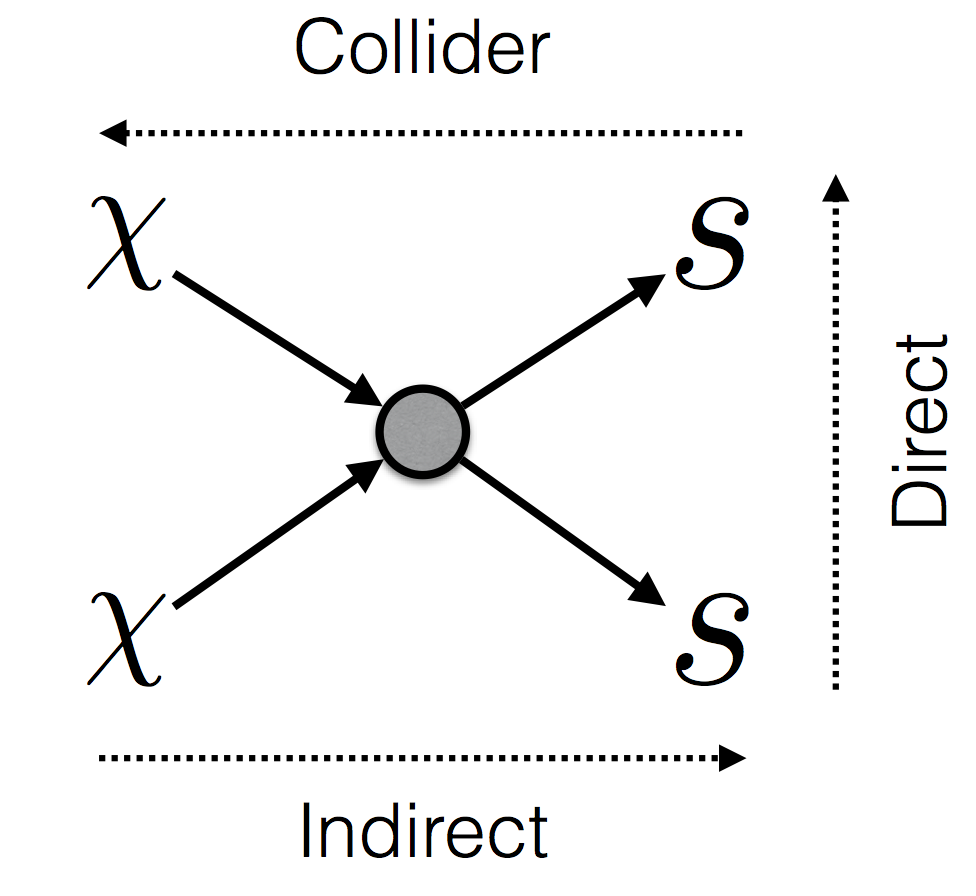
\includegraphics[width=0.65\textwidth]{images/3waystodetect/3waystodetect.pdf}
      \caption[3 Search Techniques]{
        The three general search techniques for dark matter.}
      \label{fig:3_searches}
    \end{figure}

    In Collider searches, $ss \rightarrow \chi\chi$, standard model particles ($ss$) are accelerated into each other within a detector, and the resulting particle fragments are measured by a slew of measuring equipment.
    {\color{red}Since the properties of the accelerated particles are well known (?? this is not entirely true, the interior quarks and gluons can have different momentums, sentence should be more precise -Orel)}, output fragment particles are well measured, searching for any break from {\color{red}conservation laws (?? The break from conservation laws does not yield dark matter particles. It can be used to search for them. Maybe ''suggest dark matter particles production``? --Orel)} may yield dark matter particles.
    {\color{red}This method has previously allowed for the discovery of many other new particles (?? Not accurate, most of these particles were detected directly through the particles they decayed to (like the higgs decaying to two photons). Dark matter would manifest as missing momentum since we cannot see the particles it decays to. -Orel)}, including the gluon in 1979~\cite{gluon_discovery}, the W and Z bosons in 1983~\cite{WZ_discovery1,WZ_discovery2}, the top quark in 1995~\cite{top_discovery}, the tau neutrino in 2000~\cite{tau_neutrino_discovery}, and the higgs boson in 2012~\cite{Higgs_ATLAS,Higgs_CMS}.

    With Direct searches, $\chi s \rightarrow \chi s$, sensitive particle detectors are built deep underground, where a dark matter particle impacting against an electron or nuclei creates a detectable recoil.
    Depending on the detector, this recoil can cause a detectable charge, an increase in temperature, an acoustic vibration, or a visual reaction like a photon or a gas bubble in a liquid.
    Often experiments make use of several of these signals, {\color{red}as well as the time difference between each of observable (?? what do you mean? -Orel)}.
    Though to date, no substantial dark matter signal has been detected with these methods~\cite{direct_dm_detection}.

    With Indirect searches, $\chi\chi \rightarrow ss$, astrophysical observations are analyzed for excess standard model particles, unexplained by known astrophysical processes.
    In this analysis an excess of gamma rays is sought, as the center of our galaxy is believed to host a dark matter halo.
    This spherical halo would allow for many $\chi\chi$ annihilations, producing gamma rays via: 

    $$\chi\bar{\chi} \rightarrow S\bar{S} \rightarrow \gamma\gamma$$

    where $S\bar{S}$ can be any quark or lepton particle-antiparticle pair ($t\bar{t}$, $s\bar{s}$, $e^{-}e^{+}$, etc).
    These different annhilation channels can produce different spectra of gamma rays, which will also vary based on the WIMP mass and cross-section chosen.
    This is described further in Section \ref{dm_spectral}.

\FloatBarrier

\section{Galactic Center}

  The galactic center is a complex region of space, with many astrophysical sources of gamma rays.
  A disk of dust lies along the galactic plane, acting as an interaction medium for diffuse proton cosmic rays.
  Nearby supernova remnants also produce gamma-rays as their expanding shell interacts with ambient dust.
  The immediate area surrounding the galactic center is a point-source gamma-ray emitter, though this mechanism is uncertain.

  % black hole
  Through kinematic observations of nearby stars, it was deduced that the galactic center is home to a supermassive black hole, with a mass of \SI{4e6}{\Msol}~\cite{sgra_massdist}.
  The Galactic Center also is a source of \TeV{} gamma rays, though the mechanism that produces them is still under debate.
  One possibility is that the supermassive black hole accelerates protons to PeV energies, {\color{red}which convert (?? should be more precise? -Orel)} into TeV gamma rays~\cite{gc_pevatron}.
  The second possibility suggests a nearby population of Millisecond Pulsar Wind Nebulae {\color{red}may be producing gamma rays~\cite{gc_pulsars} (?? This sentence is not really clear, are you missing a word or something? -Orel)}.
  While the Galactic Center is a source of gamma rays, the current generation of gamma-ray telescopes can only resolve it into a point source, due to their limited angular resolution {\color{red}(rewrite this!?? citation??)}.
  This analysis instead focuses on the gamma ray flux outside this point-like inner angular region.

  The disk of gas present in the galactic plane acts as an interaction medium for passing cosmic rays, both from nearby galactic accelerators and from extragalactic sources.
  {\color{red}(discuss diffuse emission??)}

  {\color{red}(somewhere in thesis cite something from each defense committee member!)}

\section{Indirect Dark Matter Search}
  For this analysis, it is important to understand how a terrestrial telescope like VERITAS can detect the presence of dark matter.
  This is done indirectly: by searching for gamma-rays that are emitted when two dark matter particles annihilate.
  As the rate of annihilation depends on the local dark matter number/volume density, the radially-dependent structure of dark matter halos also affects the analysis.

  \subsection{Dark Matter and Gamma Rays}
    {\color{red}(?? You should probably remind the reader here that WIMPs are dark matter candidates (or maybe it's cause I read the previous chapter a couple of months ago) -Orel) }
    WIMPs are predicted to decay and self-annihilate into standard model particles.
    Primarily, indirect searches focus on annihilating WIMPs, as the predicted WIMP decay lifetime produces a lower flux of standard model particles than annihilation.
    WIMPs may annihilate into {\color{red}any standard model particle (?? Should be a bit more precise. It cannot be just any SM particle, it has to be a pair of particle anti-particle or to a pair of neutral particles, etc. -Orel)}, but most studies examine a WIMP annihilating into a quark-antiquark pair, or a pair of gamma-ray photons.

    For example, two annihilating WIMPs may produce a $t\bar{t}$ pair, which then decays into... {\color{red}(?? The top decays to Wb 99.9\% of the time. -Orel)}.
    Or, they may produce $b\bar{b}$, or $\gamma\gamma$.

    These different annihilations will produce different spectra of final gamma rays.
  
  \subsection{Dark Matter Halo Structure}\label{dm_spatial}
    From observations, most galactic dark matter halos can be modeled by several similar density profiles.
    A currently favored profile is the Einasto profile~\cite{einastoprofile1,einastoprofile2}.
    This profile describes the mass/volume density of dark matter at a distance r from the halo center, $\rho(r)$.
    The Einasto profile is described by Equation \ref{eqn:einasto},

    \begin{equation} \label{eqn:einasto}
      \rho_{DM} \left( r \right) = \rho_{s} Exp \left( - \frac{2}{\alpha} \left( {\left( \frac{r}{r_s} \right)}^{\alpha} - 1 \right) \right)
    \end{equation}
    
    where the best-fit $\alpha$ is {\color{red}0.17 (?? You should say what the profile was fit to in order to obtain 0.17. -Orel)}, from~\cite{PieriGalaxySims}.
    $r_s$ is {\color{red}(and was chosen how??)}.
    $\rho_s$ is {\color{red}(and was chosen how??)}.

    Other profiles exist, but for this analysis only the Einasto profile is considered.
    Most simulations show that density profiles should terminate in a sharp peak at $r=0$ {\color{red}(?? Why is this point about how to terminate the profile important and why is it simpler to assume what you did? -Orel)}, but observations of dwarf galaxies instead favor a flat core within a given radius~\cite{CoreVsCusp}.
    For simplicity in this initial analysis, no core flattening is applied.
    
    The distance to the galactic center is fixed at \SI{8}{kpc}~\cite{gc_distance_1,gc_distance_2,gc_distance_3}, and the local estimated dark matter mass density is fixed at \SI{0.4}{\GeV\per\cm^3}~\cite{local_dm_density}, though this varies depending on the assumed Milky Way mass profile~\cite{direct_dm_astrophysical_uncertainties}.
    A scale radius $r_s$ of \SI{15.14}{kpc} {\color{red}(cite??)} is also used, and the Einasto profile for the the galactic center halo is shown in Figure \ref{fig:gchalo_density}.
  
    \begin{figure}[ht]
      \centering
      \includegraphics[width=0.95\textwidth]{images/halo/gc_einasto_profile.eps}
      \caption[Galactic Center Einasto Halo Density]{
        Mass density of the dark matter halo used in this analysis.}
      \label{fig:gchalo_density}
    \end{figure}
    
    These profiles can then be used to calculate the spatial distribution of gamma-ray {\color{red}flux (??)}.
    For annihilating dark matter, $\rho\left(r\right)^2$ must be integrated along the line of sight.
    To calculate the amount of gamma rays produced by these annihilations, Equation \ref{eqn:dmflux} can be used.
    
    \begin{equation}\label{eqn:dmflux}
      \frac{ d\Phi }{ dE d \Omega } = \frac{ \left \langle \sigma v \right \rangle }{8 \pi m_\chi^2} \frac{dN_{\gamma}}{dE} \int \rho^2 dl
    \end{equation}
    
    In this, the photon flux $\Phi$ is the number of gamma rays detected per area and per time.
    $\left \langle \sigma v \right \rangle$ is the velocity-averaged cross-section of the dark matter candidate.
    The velocity-averaging is used because the cross-section is velocity dependent, and from simulations the WIMP particles within the halo likely posesses a distribution of velocities {\color{red}(cite??)}.
    The $\frac{dN_{\gamma}}{dE}$ is the spectrum of photons produced by a single $\chi\chi$ annihilation.
    
    \begin{figure}[ht]
    \centering
      \includegraphics[width=0.95\textwidth]{images/halo/gc_einasto_jfactor.eps}
      \caption[Galactic Center Einasto Halo Jfactor]{
        J-factor profile as a function of angle from the galactic center.
        J-factor values are calculated with an integration angle of \ang{0.01}.
        {\color{red}Y axis label??}
      }
      \label{fig:gchalo_jfactor}
    \end{figure}
    
    {\color{red}Additionally (Additionally to what?? -Orel)}, simulations of galaxy formation indicate that the presence of baryons can diffuse the central cusp of particles into a core-like shape~\cite{corecusp_baryondiffuse1,corecusp_baryondiffuse2}.
    This creates a central area of constant density in the profile called a core.
    However, due to the small volume contained by this core region within most galaxies, there are comparativly few stellar emitters that can be used to precisely determine the core behavior.
    {\color{red}(Not sure what is the meant by this paragraph and how it connects to the previous one?? -Orel)}

    {\color{red}Sommerfield enhancement \url{https://arxiv.org/pdf/1005.4678.pdf} (??)}

    % from http://www.pnas.org/content/112/40/12264.full.pdf
    
    {\color{red}DM Flux skymap in galactic (l,b) ??}
    
  \subsection{Spectrum of Gamma Rays from Dark Matter}\label{dm_spectral}
    In order to calculate the brightness of the dark matter halo in gamma rays, the produced spectrum from each WIMP annihilation must be known.
    Each WIMP annihilation may directly produce two gamma rays, or may instead produce a quark-antiquark pair, a lepton-antilepton pair, or almost any other particle-antiparticle pair, called annihilation channels. 
    Non-gamma-ray annihilation channels still indirectly produce gamma rays as the pair of particles decay.
    Many standard model particle-antiparticle annihilations also result in a mix of annihilation channels, so WIMPs may also have this feature, though mixing channels tends to {\color{red}decrease the gamma-ray brightness (run this by someone else??)}, so simple single-channel annihilation spectra are searched for first.
    {\color{red}(Didn’t really follow this previous sentence's argument?? -Orel)}
    In order to calculate the different produced gamma-ray spectra for each annihilation channel, the software package CLUMPY \cite{CLUMPYcode} is used.
    The spectral models that CLUMPY uses are based on the tables in PPPC 4~\cite{pppc4_dm_spectra}.
    For this analysis, only the $b\bar{b}$ annihilation channel is considered.
    In Figure \ref{fig:chichi_spectrum}, the resultant spectra from the single annihilation of two WIMPs can be seen.
    Each line represents the spectrum from a different initial WIMP mass.

    \begin{figure}[ht]
      \centering
      \includegraphics[width=0.95\textwidth]{images/spectra/chichi_spectrum.eps}
      \caption[Single Annihilation Spectra]{
        Resultant photon spectra from a single annihilation of WIMP particles.
        Each colored line represents a different WIMP mass.}
      \label{fig:chichi_spectrum}
    \end{figure}

    These spectra, then can be combined with the {\color{red}J-factor equation (You didn’t mention what the J-factor is (and its figure is not mentioned in the text??). -Orel)} to calculate how many gamma rays are produced by the halo.

    \FloatBarrier
    
    
\section{Atmospheric Showers}

  When a particle strikes an atom of Earth's atmosphere at GeV or higher energies, it can set off a cascade of energetic particles called an air shower~\cite{Bethe1934,Klein1999}.
  When the primary particle is a gamma ray, an electron, or a positron, it creates an electromagnetic shower.
  When the primary is composed of one or more baryons, like a proton or Iron atom, it creates a hadronic shower.
  Electromagnetic showers produce a cascade of $e^{\pm}$s, $\mu^{\pm}$s {\color{red}(?? muons in an electromagnetic shower?? -Orel)}, and $\gamma$'s, where each successive generation of particles tends to have more particles but less energy per particle than the last.
  To start the shower, the primary gamma ray will interact with an atmospheric atom, producing a $e^{-}e^{+}$ pair, each with roughly half the primary gamma ray's energy, as shown in Figure \ref{fig:emcascade}.
  The $e^{-}$ and $e^{+}$ may emit some photons as bremstrahlung radiation, and then {\color{red}collide with other atmospheric atoms to produce more $e^{-}e^{+}$ pairs (?? The photons are the ones which produce more e+e- pairs -Orel)}.
  As each newly created particle has less energy than its parent particle, eventually the particles in the shower don't have enough energy to produce additional child-particles.
  This occurs when electrons have around \SI{80}{MeV} of kinetic energy, where they rapidly lose energy to ionization~\cite{pdg_2014}.

  \begin{figure}[ht]
    \centering
    \includegraphics[width=0.85\textwidth]{images/cascade_diagram/emcascadegv.pdf}
    \caption[Electromagnetic Cascade]{
      Diagram of an electromagnetic cascade as it decends downwards through the atmosphere, layered by interaction generation.
      $\gamma{}o$ is the initial astrophysical gamma ray, and continues for many generations after these first four.
      {\color{red}(?? Only gamma's should pair produce, leptons should only bremstrahlung, since leptons only pair-convert when they're below the 80MeV.)}
      {\color{red}(?? Photons are bosons, in feynman diagrams should have wiggly lines!)}
    }
    \label{fig:emcascade}
  \end{figure}

  \begin{figure}[ht]
    \centering
    \feynmandiagram[horizontal=a to b]{
      i1 -- [fermion] a -- [fermion] i2,
      a  -- [photon]  b,
      f1 -- [fermion] b -- [fermion] f2
    };
    \caption[em1test]{em1test}
    \label{fig:em1test}
  \end{figure}
  
  \begin{figure}[ht]
    \centering
    \feynmandiagram[horizontal=i0 to a]{
      i0 -- [photon , edge label=\(\gamma\)] a,
      a  -- [fermion, edge label=\(e^{+}\) ] b,
      a  -- [fermion, edge label=\(e^{-}\) ] c 
    };
    \caption[em2test]{em2test}
    \label{fig:em2test}
  \end{figure}
  
  As most (\nicetilde 99\%) of detected air showers are due to {\color{red}protons and not gamma rays (what about electron showers??)}, understanding the differences between hadronic and electromagnetic showers becomes useful in removing unwanted proton events and preserving gamma-ray events within the reconstruction method, sometimes referred to as gamma-hadron separation.
  Hadronic showers start with a primary \nicetilde TeV proton that interacts with an atmospheric atom.
  {\color{red}This proton then converts (?? It doesn't convert to pions. Definately not to pi+ pi- adn pi0, (charge conservation). -Orel)} into $\pi^{+}$, $\pi^{-}$, and $\pi^{0}$, each with roughly \nicetilde $\frac{1}{3}$ of the initial proton's energy.
  {\color{red}(?? Isn't there also a neutron in some diagrams??)}
  % see here for neutron: https://en.wikipedia.org/wiki/Cosmic_ray
  The $\pi^{+}$ and $\pi^{-}$ can travel far in the tranverse direction, away from the main axis of the primary particle, then decay into $\mu^{+}\nu_{\mu}$ and $\mu^{-}\bar{\nu}_{\mu}$ pairs, respectivly.
  The $\pi^{0}$ quickly decays into $\gamma\gamma$, which then each start their own electromagnetic shower.
  The $\pi^{+}$ and $\pi^{-}$ have longer decay time ($\pi^{\pm} \rightarrow $\SI{3e-8}{s} vs $\pi^{0} \rightarrow $\SI{9e-17}{s} \cite{pdg_2014} ), allowing them to carry energy further away from the central shower axis.
  Both of these effects contribute to sub-showers being created further away from the primary particle axis, which tends to cause hadronic showers (and their resulting Cherenkov images, discussed in Section \ref{sec:cherenkov}) to be wider than a purely electromagnetic shower of the same length. 
  
  In Figure \ref{fig:gamma_vs_proton_airshower}, the differences between a gamma-ray shower and a proton shower are shown.
  The gamma-ray shower on the left has most of its particles along the veritical core of the shower, while the proton shower has more particles spread out in a wider, fan-like shape.
  The initial energies were chosen as a \SI{1}{TeV} proton shower will on average divest $\frac{1}{3}$ of its energy to the $\pi^{0}$, which then decays into an electromagnetic sub-shower depicted in the image, so these two showers have roughly the same initial available energy.

  \begin{figure}[ht]
    \centering
    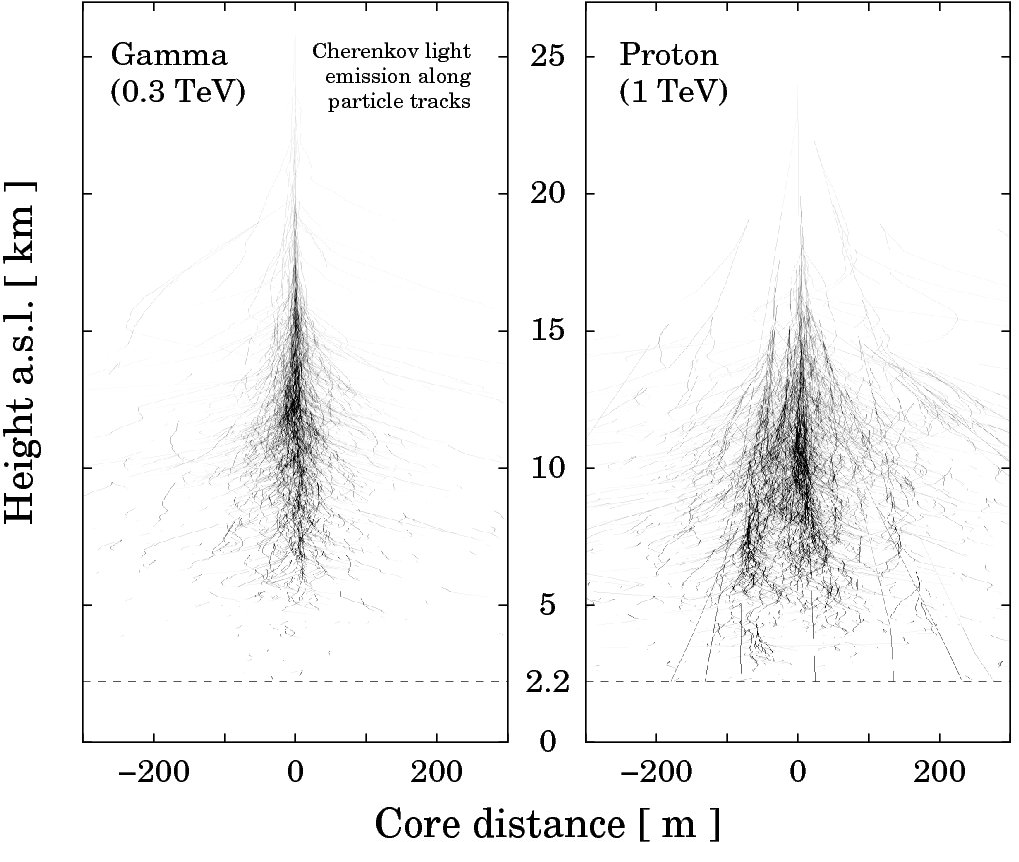
\includegraphics[width=0.95\textwidth]{images/showers_gamma_proton}
    \caption[Gamma Ray and Proton Showers]{
      A gamma ray shower alongside a proton shower~\cite{Bernlohr2008149}.
    }
    \label{fig:gamma_vs_proton_airshower}
  \end{figure}
  
  \FloatBarrier

  \subsection{Cherenkov Photons}\label{sec:cherenkov}

  Within atmospheric showers, any charged particles travelling at velocity $v > c_{atmosphere}$ will induce the atmosphere to produce Cherenkov photons~\cite{cherenkov}, where $c$ is the speed of light in the atmosphere.
  From a single charged particle of constant velocity, Cherenkov photons form a conical wavefront shown in Figure \ref{fig:cherenkovangle}, similar to a sonic boom shockwave or the wake produced when a boat travels faster than the speed of the waves.

  \begin{figure}[ht]
    \centering
    \includegraphics[width=0.27\textwidth]{images/cherenkov_angle/cherenkovangle.eps}
    \caption[Chernekov Emission Angle]{
      Cherenkov light (blue arrows) is emitted at angle $\theta$, relative to its the charged particle z's path.
    }
    \label{fig:cherenkovangle}
  \end{figure}

  Cherenkov photons are produced at an angle $\theta$ relative to the charged particle's path, determined by the index of refraction of the medium $n$, the speed of the charged particle $v$, and the speed of light in the medium $c$, as in Equation \ref{eqn:cherenkovangle}.

  \begin{equation}\label{eqn:cherenkovangle}
    \theta = ArcCos \left ( \frac{c}{n \; v} \right )
  \end{equation}
  
  For the gamma-ray showers used in this analysis, the cherenkov angle is \nicetilde\ang{1}.
  % showers are 10km up, light pool on ground is 130m diameter, \theta = ArcSin(130/10000) * 180 / pi = 0.73deg ~ 1deg

  However in an atmospheric shower, the number and distribution of charged particles and their velocities, as well as energy losses, tend to smear the theoretically-clean Cherenkov cones into a diffuse pool of light on the ground.
  
  Cherenkov photons are produced with a spectrum following the Frank-Tamm formula~\cite{franktamm1,franktamm2} in Equation \ref{eqn:franktamm}.
  
  \begin{equation}\label{eqn:franktamm}
    \frac{dE}{dx\,d\omega}=\frac{(ze)^2 \, \omega}{c^2} \left ( 1 - \frac{c^2}{v^2 \;\epsilon(\omega)} \right )
  \end{equation}
  
  Where $E$ is the energy emitted as Cherenkov radiation, $x$ is the length of the charged particle path, $ze$ is the charge of the particle, $\omega$ is the emitted Cherenkov photon frequency, $c$ is the speed of light (phase velocity) in the medium, $v$ is the speed of the particle, and $\epsilon(\omega)$ is the frequency-dependent permittivity.
  The UV- and Visible-spectrum Cherenkov photons are then imaged and recorded by the VERITAS observatory.
  {\color{red}(Why just those frequencies?? does the cerenkov spectrum cutoff, or atmospheric absorption??)}
  {\color{red}(?? I think UV is absorbed by the atmosphere almost completely no?  Either way, those are the frequencies imaged because they are the ones Cherenkov light -Orel)}
  
  \begin{figure}[ht]
    \centering
    \includegraphics[width=0.75\textwidth]{images/CherenkovReactor/cherenkovreactor.eps}
    \caption[Chernekov Light from a Reactor]{
      Blue Cherenkov light in the Advanced Test Rector core, at the Idaho National Laboratory~\cite{cherenkovreactor,atrlab}.
    }
    \label{fig:cherenkovreactor}
  \end{figure}
  In Figure \ref{fig:cherenkovreactor}, a visible example of Cherenkov photons is shown, produced in the Advanced Test Reactor at the Idaho National Laboratory.
  Neutrons emitted by the reactor collide with atoms in the water, freeing some electrons with enough kinetic energy to travel faster than the speed of light in water, which then create the blue Cherenkov photons imaged here.
  
  {\color{red}(image of cherenkov light pool on ground??)}
  {\color{red}(?? Orel agrees with this!)}
  
  
